% !TEX program = xelatex
\documentclass[sigconf,nonacm]{acmart}

\usepackage{kotex}
\usepackage{graphicx}
\usepackage{booktabs}
\usepackage{array}
\usepackage{enumitem}
\usepackage{balance}
\setlist[itemize]{leftmargin=*,nosep}
\settopmatter{printacmref=false, printccs=false, printfolios=true}
\renewcommand\footnotetextcopyrightpermission[1]{}
\pagestyle{plain}

\title{TaskSense: LLM으로 이기종 센서 시스템에 작업을 지시하기 위한 번역 유사 접근법}
\author{Kaiwei Liu, Bufang Yang, Lilin Xu, Yunqi Guo, Guoliang Xing, Xian Shuai, Xiaozhe Ren, Xin Jiang, Zhenyu Yan}
\affiliation{\institution{SenSys 2025}}
\email{}

\begin{document}
\maketitle

\begin{abstract}

스마트홈과 공장 같은 환경에는 다양한 지능형 애플리케이션을 가능하게 하기 위해 여러 센서 시스템이 점점 더 많이 설치되고 있다. 하지만 기존의 센서 조정 시스템 대부분은 사람이 미리 정의한 규칙에 의존하므로, 유연하고 복잡한 작업을 처리하는 데 한계가 있다. 최근에는 대규모 언어 모델(LLM)을 사용해 외부 API와 상호작용하는 접근법이 등장했지만, 실제 센서 시스템의 기능과 데이터 의존성을 충분히 이해하는 데 어려움을 겪는다.
\end{abstract}
\begin{figure}[t]
  \centering
  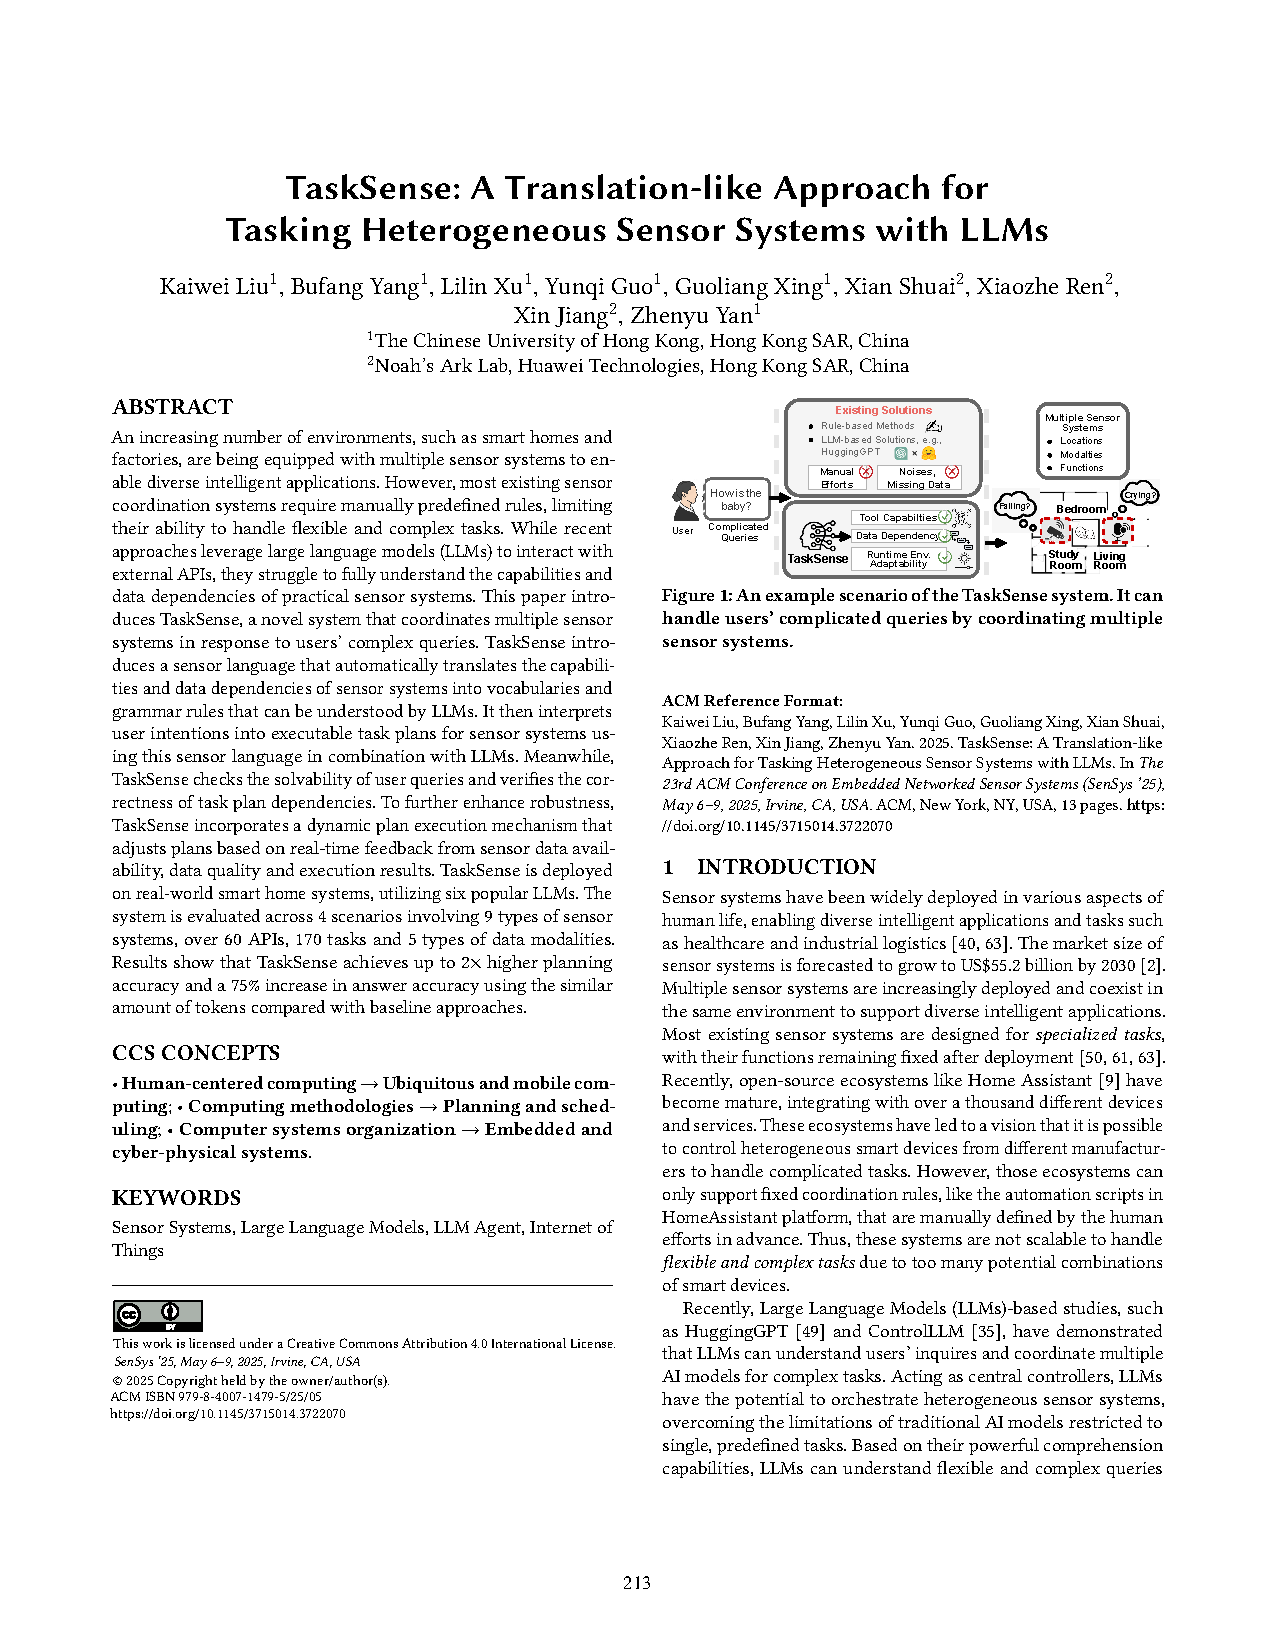
\includegraphics[page=1,width=\columnwidth,trim={310bp 477bp 32bp 105bp},clip]{sensys_tasksense.pdf}
  \caption{An example scenario of the TaskSense system.}
\end{figure}


이 논문은 사용자의 복잡한 질의에 응답하기 위해 여러 센서 시스템을 조정하는 새로운 시스템인 TaskSense를 제안한다. TaskSense는 센서 시스템의 기능과 데이터 의존성을 LLM이 이해할 수 있는 어휘와 문법 규칙으로 자동 변환하는 센서 언어(sensor language)를 도입한다. 이후 이 센서 언어와 LLM을 결합해 사용자 의도를 센서 시스템이 실행할 수 있는 작업 계획으로 해석한다.

TaskSense는 사용자 질의가 해결 가능한지 검사하고, 작업 계획의 의존성이 올바른지도 검증한다. 또한 강건성을 높이기 위해 센서 데이터의 가용성, 데이터 품질, 실행 결과에 대한 실시간 피드백을 바탕으로 계획을 조정하는 동적 계획 실행 메커니즘을 포함한다.

TaskSense는 실제 스마트홈 시스템에 배포되었고, 여섯 가지 인기 LLM을 사용해 평가되었다. 평가는 4개 시나리오, 9종 센서 시스템, 60개 이상의 API, 170개 작업, 5종 데이터 모달리티를 포함한다. 결과적으로 TaskSense는 기존 방법과 비슷한 토큰 수를 사용하면서도 계획 정확도를 최대 2배 높이고, 응답 정확도를 75\% 향상시켰다.

\section{1. 서론}

센서 시스템은 헬스케어, 산업 물류 등 다양한 지능형 애플리케이션과 작업을 가능하게 하며 인간 생활 전반에 널리 배포되고 있다. 센서 시스템 시장 규모는 2030년까지 552억 달러에 이를 것으로 전망된다. 하나의 환경 안에 여러 센서 시스템이 공존하면서 다양한 지능형 애플리케이션을 지원하는 경우도 늘고 있다.

기존 센서 시스템 대부분은 특정 작업에 맞게 설계되며, 배포 이후 기능이 고정된다. 최근 Home Assistant 같은 오픈소스 생태계는 성숙해졌고, 천 개 이상의 기기와 서비스를 통합한다. 이런 생태계는 서로 다른 제조사의 이기종 스마트 기기를 제어해 복잡한 작업을 처리할 수 있다는 비전을 보여준다. 하지만 현재 이러한 생태계는 사람이 사전에 수동으로 정의한 고정 조정 규칙만 지원한다. 따라서 가능한 스마트 기기 조합이 너무 많아지면, 유연하고 복잡한 작업을 확장성 있게 처리하기 어렵다.

최근 HuggingGPT, ControlLLM 같은 LLM 기반 연구는 LLM이 사용자의 질의를 이해하고 여러 AI 모델을 조정해 복잡한 작업을 수행할 수 있음을 보였다. LLM은 중앙 제어기 역할을 하며, 사전에 정의된 단일 작업에 제한되는 기존 AI 모델의 한계를 넘어 이기종 센서 시스템을 오케스트레이션할 가능성이 있다. LLM의 강력한 이해 능력은 자연어로 표현된 유연하고 복잡한 질의를 해석하고, 사용자 의도에 맞는 계획을 생성하고, 실행 결과를 사용자 친화적인 응답으로 번역할 수 있게 한다.

그러나 기존 LLM 기반 조정 솔루션은 주로 AI 모델이나 알고리즘 호출에 초점을 맞추며, 실제 센서 시스템을 조정하는 데에는 부족하다. 실제 센서 시스템의 기능과 기능 모듈 사이의 데이터 의존성에 대한 지식이 부족하기 때문에, 사용자 질의의 해결 가능성을 정확히 판단하거나 센서 시스템을 올바르게 조정하지 못한다. 또한 현실 환경의 불확실성 아래 안정적인 성능을 유지하기 어렵다.

예를 들어, 집에 영상 감시 시스템과 스마트 스피커가 설치되어 있고 사용자가 아기의 잠재적 이상 상태를 모니터링하고 싶다고 하자. 아기가 넘어지는 것이 감지된 뒤 울면 시스템은 사용자에게 경고해야 한다. 이런 질의는 여러 센서 시스템의 다양한 조합을 요구하며 동적으로 변한다. 다른 예로는 “어제 방 안에 누가 있었나?”, “내 열쇠가 어디 있지?” 같은 질의가 있다.

이 논문은 도구의 기능과 도구 간 의존성을 충분히 이해해 하나 이상의 센서 시스템을 조정하는 LLM 기반 시스템 설계를 탐구한다. 여기서 도구(tool)는 데이터 처리, 센서 제어처럼 센서 시스템 안의 특정 기능 모듈을 뜻한다. 하지만 이러한 작업 지시 시스템을 설계하려면 몇 가지 문제가 있다.

첫째, 센서 시스템이 배포된 뒤 조정 시스템은 다양한 도구 기능을 이해해야 한다. 기능에는 특화 AI 모델, 데이터베이스 연산, 센서 제어, 데이터 전송 등이 포함될 수 있다. 각 도구의 능력 한계와 복잡한 상호 의존성을 이해하는 것은 LLM에게 어렵다. 예를 들어 감시 카메라 시스템은 이상 행동을 감지할 수 있지만 개인을 식별하지는 못할 수 있다. 반대로 얼굴 인식 도구는 센서가 직접 촬영한 전체 이미지가 아니라 잘려진 얼굴 이미지만 입력으로 받을 수 있다.

둘째, 실제 환경 변화는 데이터 품질과 가용성에 큰 영향을 주고, 조정 실패를 일으킬 수 있다. 동일한 작업을 완료하기 위해 실행 중에 도구를 동적으로 교체해 대체 계획을 자동 생성하는 것은 어렵다.

TaskSense는 센서 언어라는 특수 프레임워크를 사용해 LLM이 센서 시스템과 상호작용하도록 하는 번역 기반 접근법이다. 센서 시스템이 배포되면, TaskSense는 그 기능을 LLM이 이해할 수 있는 어휘와 문법으로 자동 변환한다. 사용자가 질의를 제출하면 TaskSense는 먼저 해결 가능성을 검사하고, 센서 언어를 바탕으로 사용자 의도를 실행 가능한 계획으로 변환한다. 이후 문법 검사를 통해 계획의 의존성 오류를 탐지한다. 실행 중에는 센서 데이터 품질, 데이터 가용성, 실행 결과의 피드백에 따라 계획을 동적으로 조정한다. 마지막으로 센서 시스템의 출력을 자연어로 다시 번역해 사용자에게 명확한 응답을 제공한다.

이 논문의 기여는 다음과 같다.

\begin{itemize}
\item 이기종 센서 시스템을 LLM이 조정해 복잡한 사용자 질의를 수행하도록 하는 첫 번째 번역 유사 접근법인 TaskSense를 개발했다.
\item 센서 시스템의 기능 경계와 기능 모듈 간 관계를 LLM이 이해하도록 어휘 집합과 문법을 정의하는 새로운 센서 언어를 제안했다. 이를 통해 실행 가능한 계획을 자동 생성하고, 작업 해결 가능성과 데이터 의존성을 보장한다.
\item 런타임 환경 불확실성을 다루기 위해 센서 시스템 조정을 위한 동적 계획 적응 메커니즘을 설계했다. 센서 실패, 데이터 품질, 실행 결과를 바탕으로 실행 경로를 조정한다.
\item 4개 데이터셋에서 TaskSense를 구현했다. 평가에는 9개 센서 시스템, 60개 이상의 API, 170개 작업, 5종 데이터 모달리티가 포함된다. 기존 최신 솔루션과 비슷한 토큰 수를 사용하면서 계획 정확도는 최대 3배, 응답 정확도는 1.75배 향상되었다.
\end{itemize}


\section{2. 관련 연구}

\subsection{2.1 센서 시스템 작업 지시}

다양한 스마트 센서 시스템은 일상생활에 통합되어 왔다. 전통적인 센서 시스템은 규칙 기반 작업 실행 전략에 의존한다. ADMarker는 노인의 집에 다양한 센서와 AI 모델을 결합해 초기 알츠하이머병을 감지한다. Kratos+는 정책 협상 알고리즘으로 여러 센서를 관리해 다양한 사용자 요청을 충돌 없이 처리한다. 하지만 이러한 솔루션은 사전에 정의된 고정 작업에 제한되며, 동적인 사용자 요구에 적응하지 못한다.

최근 연구는 임베디드 시스템의 복잡한 작업을 해결하기 위해 LLM을 활용한다. 일부 연구는 LLM으로 AI 모듈과 IoT 기기에 작업을 할당해 다양한 사용자 요구를 만족시킨다. Sasha는 LLM을 사용해 홈 디바이스를 관리하고 개방형 지시에 대한 행동 계획을 생성한다. 하지만 이러한 솔루션은 센서 시스템에 작업을 지시할 때 환경 불확실성을 고려하지 않아, 실제 애플리케이션에서 강건성이 제한된다.

\subsection{2.2 작업 계획을 위한 LLM}

일부 연구는 LLM을 의사결정 중심으로 사용해 외부 도구를 호출하고 복잡한 작업을 해결한다. ToolFormer는 LLM이 외부 도구 API 사용법을 학습해 더 신뢰할 수 있는 답을 생성할 수 있음을 보였다. HuggingGPT와 TaskMatrix.AI는 LLM을 제어기로 사용해 작업 해결 계획을 제안하고 각 단계에 맞는 도구를 선택한다. ToolLLM과 ControlLLM은 가능한 계획 중 최적 계획을 찾기 위해 각각 트리 기반 및 그래프 기반 탐색 방법을 사용한다.

하지만 이런 시스템은 계산기, 위키백과, 특화 AI 모델 같은 일반 도구 호출에 초점을 맞추며, 실제 센서 시스템의 복잡한 환경과 데이터 의존성을 고려하지 않는다.

LLM의 계획 품질을 개선하려는 연구도 있다. Self-check는 추가 LLM을 검증기로 사용해 단계별 추론 과정의 오류를 인식한다. ToolLLM과 KwaiAgents는 고품질 지시 데이터셋으로 LLM을 파인튜닝해 계획 능력을 높인다. TaskMatrix.AI와 Sasha는 사용자 피드백을 사용해 계획 품질을 개선한다. Voyager와 LLMind는 프로그램 실행 오류를 피드백으로 사용한다. 일부 연구는 객관적 환경에서 얻은 관찰을 LLM에 결합하려 시도한다. 하지만 이런 방법은 추가 검증기에 의존하거나, 실행 오류 및 사람 피드백에 기대며, 센서 시스템 자체의 정보를 충분히 활용하지 못한다.

\subsection{2.3 센서 시스템의 개방형 질의응답을 위한 LLM}

M4와 OneLLM은 대량의 멀티모달 센서 데이터로 어댑터를 학습해 원시 센서 데이터를 LLM 임베딩 공간으로 매핑한다. 이를 통해 센서 데이터 기반 개방형 질의응답을 수행할 수 있다. 하지만 다양한 센서 데이터 모달리티를 자연어 임베딩 공간에 맞추려면 많은 학습 데이터가 필요하고, 특히 IMU처럼 복잡하고 정보가 희소한 모달리티에서는 어렵다.

다른 연구들은 임베디드 시스템 안에서 센서 데이터 추론을 위한 LLM 능력을 탐구한다. LLMTrack은 Chain-of-Thought 프롬프팅으로 IMU 데이터를 분석해 궤적을 인식하고, LLMSense는 인간 활동 인식 모델의 일상 활동 로그에 대해 고수준 추론을 수행한다. RAG 기법으로 환자의 일상 웨어러블 데이터 같은 외부 지식베이스에 접근하는 연구도 있다.

하지만 이러한 시스템에는 두 가지 큰 한계가 있다. 일부는 데이터 로그를 갱신하기 위해 여러 작업 특화 모델을 지속 실행해야 하므로 계산 자원과 유연성 문제가 크다. 다른 일부는 센서 데이터 이해와 추론에 주로 집중해 더 넓은 작업 유형을 다루지 못한다.

\section{3. 동기}

이 절은 현재 센서 시스템 작업 지시 방법을 세 단계로 살펴본다. 첫째, 사용자 질의에 따라 도구 호출 계획을 생성한다. 둘째, 계획을 실행한다. 셋째, 실행 결과에서 응답을 전달한다. 기존 접근법과 실제 테스트베드에서 얻은 관찰이 TaskSense 설계 목표를 이끈다.

\subsection{3.1 질의로부터 계획 생성}

기존 센서 시스템이 실제 사용자 질의를 처리하는 능력을 이해하기 위해, 저자들은 가정 내 노인 돌봄 시나리오에서 최신 접근법인 HuggingGPT를 테스트했다. 이 시나리오에서는 홈 감시 시스템, 심층 행동 인식 시스템, 소리 감지 시스템 등 여러 센서 시스템이 노인의 집에 배치되어 일상 활동을 모니터링하고 기록한다. MDS-UPDRS에서 유도한 인간 활동 및 감정 관련 임상 질의 38개를 구성했고, 3개 센서 시스템의 19개 도구 중에서 LLM이 각 질의에 맞는 계획을 만들도록 했다.
\begin{figure}[t]
  \centering
  \includegraphics[page=3,width=\columnwidth,trim={315bp 622bp 47bp 80bp},clip]{sensys_tasksense.pdf}
  \caption{Distribution of planning errors using HuggingGPT for tasks in elderly care scenario.}
\end{figure}


오류는 주로 다음 세 가지였다.

\noindent\textbf{1.} 해결 가능성 오판: 현재 접근법은 도구 집합의 능력 한계를 인식하지 못하고, 도구가 처리할 수 없는 질의도 해결 가능하다고 판단하는 경우가 많다. 예를 들어 “Bob의 혈당을 요약해줘”라는 질의가 있는데 혈당 모니터링 도구가 없다면 처리할 수 없다. 또는 인간 활동 인식 도구가 “앉기”, “춤추기” 라벨은 있지만 “체스 두기” 라벨은 없을 수 있다. 이런 경우 시스템은 오해를 부르는 계획을 생성하지 말고 처리할 수 없다고 알려야 한다.\par
\noindent\textbf{2.} 잘못된 계획: 생성된 계획에 잘못된 의존성이나 잘못된 도구가 포함된다. 각 도구는 고유한 기능과 입출력 요구사항을 가지므로, 도구 간 데이터 의존성이 제한된다. 예를 들어 얼굴 표정 인식 도구는 얼굴 이미지를 입력으로 요구하므로 얼굴 감지 도구 뒤에만 올 수 있다. 얼굴 감정 인식이나 화자 분리 도구 뒤에 오면 입력이 맞지 않아 결과가 틀린다. 또한 수면 질 질의에 낙상 감지 도구를 넣는 것처럼 부적절한 도구 선택도 발생한다.\par
\noindent\textbf{3.} 형식 오류: 계획 출력 형식이 기대 형식과 맞지 않는 오류도 발생한다.\par

HuggingGPT 기반 실험에서 가장 많은 오류는 도구 집합의 능력 경계를 넘는 질의를 정확히 인식하지 못하는 데서 발생했다. 잘못된 의존성은 도구 사이의 유효한 의존성을 판단하기 어렵기 때문에 생기고, 잘못된 도구 선택은 사용자의 다양한 표현 방식을 이해하기 어렵기 때문에 발생한다.

\subsection{3.2 계획 실행과 응답}

계획을 만든 뒤에는 이를 실행하고 사용자에게 응답해야 한다. 저자들은 스마트홈 시나리오에서 HuggingGPT 프레임워크를 사용해 계획 실행 품질을 실험했다. 질의는 “Bob이 오늘 충분한 화장실 휴식 없이 과로했는가?”였고, 같은 질의에 대해 세 가지 센서 시스템에서 서로 다른 계획을 실행했다.
\begin{figure}[t]
  \centering
  \includegraphics[page=4,width=\columnwidth,trim={50bp 492bp 312bp 90bp},clip]{sensys_tasksense.pdf}
  \caption{An illustration about environmental impacts on sensor systems.}
\end{figure}


실험 결과, 환경 변화에 따라 각 계획의 성능이 달라졌다. RGB 카메라 기반 홈 감시 시스템은 나쁜 조명 조건과 가림 때문에 후반 구간에서 올바른 결과를 만들지 못했다. 심층 행동 인식 시스템과 위생 모니터링 시스템도 각각 가림이나 대상이 프레임 밖에 있는 문제 때문에 특정 구간에서 정확하지 않았다. 이는 계획 자체가 맞더라도 실행 결과가 환경 요인에 매우 민감하다는 것을 보여준다.

환경 요인은 계획 실행 경로마다 다르게 작용한다. 어떤 시스템은 특정 시간대에 대상을 감지하지 못했지만, 다른 시스템은 동일 작업을 완료할 수 있었다. 이는 센서 시스템 사이에 높은 상보성이 있음을 보여준다.

계획 실행에 영향을 주는 주요 환경 요인은 세 가지다.

\noindent\textbf{1.} 데이터 누락: 센서 고장이나 실수로 센서가 꺼지는 경우 필요한 데이터가 기록되지 않아 실행 실패로 이어진다.\par
\noindent\textbf{2.} 데이터 노이즈: RGB 카메라의 조명 변화, 음성 수집의 소음처럼 센서 데이터 품질을 낮추는 요인이 실행 결과 오류를 만든다.\par
\noindent\textbf{3.} 콘텐츠 관련 문제: 객체가 카메라 프레임 밖으로 나가거나, 가려지거나, 감지하기 어려운 자세를 취하는 경우 데이터 노이즈만으로는 판단하기 어렵지만 결과 정확도에 큰 영향을 준다.\par

이 문제를 다루려면 서로 다른 센서 사이의 상보성을 활용하는 전략이 유망하다. 예를 들어 조명 조건은 RGB 카메라 기반 도구에는 영향을 주지만 깊이 카메라 기반 도구에는 영향이 작다. 집 안 여러 위치와 각도에 인간 감지 센서를 배치하면, 사용자의 위치에 따라 다른 센서를 사용하는 계획으로 전환해 감지 결과를 보장할 수 있다. 따라서 실행 경로를 적응적으로 전환하면 환경 불확실성 영향을 줄이고 시스템 강건성을 높일 수 있다.

응답 생성 단계에도 문제가 있다. 여러 센서 시스템은 실행 중 상당한 양의 결과 데이터를 만든다. LLM은 긴 데이터 시퀀스를 처리하고 복잡한 계산을 수행하는 데 어려움을 겪어, 도구 간 잘못된 데이터 연결 같은 환각이나 망각 문제를 일으킬 수 있다. 저자들이 30개 테스트 질의로 GPT-4를 실험한 결과, 5개는 서로 다른 도구 결과의 잘못된 연결 때문에 실패했고, 3개는 불완전한 답을 생성했다. 따라서 생성 답변의 정확성을 보장하는 전략이 필요하다.

\section{4. 시스템 개요}

TaskSense는 센서 언어를 도입하고, LLM으로 센서 시스템을 조정해 동적 환경에서 사용자 질의를 이해하고 응답하는 이기종 센서 시스템 작업 지시 접근법이다.
\begin{figure*}[t]
  \centering
  \includegraphics[page=5,width=\textwidth,trim={45bp 577bp 227bp 75bp},clip]{sensys_tasksense.pdf}
  \caption{System overview of TaskSense.}
\end{figure*}


TaskSense는 먼저 LLM 기반 센서 시스템 자동 등록 방법을 사용해 어휘 집합, 문법, 시드 예제를 초기화한다. 이를 통해 시스템 초기화와 업데이트에 필요한 수작업을 줄인다. 사용자의 질의를 받으면, TaskSense는 센서 언어와 검색된 예제를 바탕으로 사용자 의도를 해석하고, 센서 시스템을 조정하기 위한 실행 가능한 도구 호출 계획으로 변환한다. 계획이 생성된 뒤에는 동적 계획 적응 메커니즘으로 런타임 실행 경로를 조정해 환경 변화와 임베디드 시스템 간섭에 강건하게 만든다. 마지막으로 계획 실행 결과를 바탕으로 센서 언어를 자연어 피드백으로 다시 번역한다.

\section{5. TaskSense 설계}

\subsection{5.1 센서 언어로 시스템 이해하기}

\subsubsection{5.1.1 센서 언어 정의}

TaskSense에서 사용자 질의는 자연어 형태로 입력되며, 센서 시스템 도구를 직접 실행하는 데 사용할 수 없다. 이 간극을 메우기 위해 저자들은 LLM의 번역 능력을 활용해 사용자 의도를 실행 가능한 도구 호출 계획으로 변환하는 번역 유사 솔루션을 개발했다.
\begin{figure}[t]
  \centering
  \includegraphics[page=5,width=\columnwidth,trim={388bp 577bp 40bp 75bp},clip]{sensys_tasksense.pdf}
  \caption{An example of vocabulary set.}
\end{figure}

\begin{figure}[t]
  \centering
  \includegraphics[page=5,width=\columnwidth,trim={45bp 427bp 312bp 220bp},clip]{sensys_tasksense.pdf}
  \caption{An example of sensor grammar.}
\end{figure}


TaskSense는 도구와 도구 간 의존성을 하나의 언어로 개념화하고 이를 센서 언어라고 부른다. 이 관점에서 도구는 센서 언어의 어휘이고, 의존성은 문법이며, 계획은 문법 규칙을 따라 어휘를 조합해 만든 문장이다. 센서 언어에는 어휘 집합과 문법 규칙이라는 두 핵심 정의가 있다. 이들은 검색된 예제와 함께 LLM 프롬프트에 포함되어 사용자 의도를 효과적으로 번역하게 한다.

센서 어휘 집합은 실행 가능한 계획을 만들 때 LLM이 사용할 수 있는 모든 도구와 기본 요소의 상세 정보를 정의한다. 각 도구의 어휘에는 범주, 도구 이름, 모달리티, 장치, 기능 설명, 입력, 출력, 출력 라벨 설정이 포함된다. 예를 들어 인간 활동 인식 도구는 비디오 속 사람의 활동을 감지하고, RGB 비디오 경로 리스트를 입력으로 받아 각 비디오의 라벨 리스트를 출력한다. PTZ 프리셋 위치 이동 도구는 지정된 카메라의 각도를 사전 설정 위치로 조정하고, 카메라 ID와 위치 ID를 입력으로 받아 성공 또는 실패 상태를 출력한다.

센서 문법은 각 계획이 따라야 하는 도구 간 의존성 규칙을 정의한다. 센서 문법은 방향 비순환 그래프(DAG)의 집합으로 구성된다. 노드는 도구를, 엣지는 도구 간 유효한 의존성을 나타낸다. LLM 프롬프트에 포함할 때 그래프는 노드 리스트와 엣지 리스트로 변환된다. 각 유효 계획은 센서 문법의 부분 그래프다.

센서 문법에는 데이터 의존성과 제어 의존성 두 종류가 있다. 데이터 의존성은 도구 사이의 데이터 입출력 관계를 정의한다. 어떤 도구는 다른 도구의 출력을 입력으로 필요로 하므로, 실행 가능한 계획이 제한된다. 이 의존성은 LLM이 생성한 계획을 검증하는 데 쓰인다. 제어 의존성은 도구의 잠재적 실행 전제조건을 정의한다. 예를 들어 RGB 인간 감지 도구가 적어도 한 사람을 감지해야 화자 분리 도구가 실행될 수 있다. 생성된 계획이 데이터 의존성 검증을 통과하면, 제어 의존성은 계획 실행 전에 자동 삽입된다.

센서 어휘와 문법은 LLM이 사용자 질의를 실행 가능한 계획으로 번역하는 데 필수적이다. 어휘는 도구 집합의 기능 경계를 정의하고, 문법은 도구 간 의존성 규칙을 지정한다. 새 애플리케이션 시나리오에 TaskSense를 적용할 때는 먼저 어휘 집합과 문법을 만들어야 한다. 기존 HuggingGPT나 Sasha는 도구 집합을 수동으로 만들어야 하지만, TaskSense는 자동 초기화를 지원한다.

구체적으로 사용자는 소프트웨어 도구의 소스 코드나 제조사가 제공하는 센서 시스템 API 설명을 제공한다. TaskSense는 새 어휘의 형식을 프롬프트에 지정한다. 새 어휘는 JSON 객체 리스트이며, 각 객체는 범주, 도구 이름, 모달리티, 설명, 입력, 출력, 라벨 설정을 가진다. 또한 5-6개의 사전 정의된 어휘 예시를 함께 제공해 LLM이 형식을 이해하게 한다. 이후 LLM은 새 도구 전체에 대한 어휘를 생성한다.

문법 규칙도 비슷하게 생성한다. TaskSense는 문법 규칙을 문자열 리스트로 구성하도록 프롬프트에 명시한다. 각 문자열은 “Face Detection -> Face Recognition”처럼 두 도구 이름을 화살표로 연결해 의존성을 나타낸다. LLM이 생성한 문법 규칙은 각 도구 쌍의 입력과 출력을 바탕으로 유효한지 검사된다. 사용자는 새 어휘나 문법 규칙을 수동으로 추가하거나 삭제할 수도 있다.

\subsubsection{5.1.2 예제 라이브러리}

어휘 집합과 문법 규칙만 제공하는 것은 센서 언어 학습에 충분하지 않다. 기계 번역에서는 병렬 말뭉치라는 예제 라이브러리를 사용해 번역 예제를 구성한다. TaskSense는 이를 센서 언어에 적용해 각 예제를 질의-계획 쌍으로 설계한다. 각 쌍은 사용자 질의 예시와 이를 해결하는 대응 계획을 포함한다. LLM은 이 예제에서 사용자 질의를 도구 호출 단계로 분해하고 실행 가능한 계획으로 구성하는 법을 배운다.
\begin{figure}[t]
  \centering
  \includegraphics[page=6,width=\columnwidth,trim={325bp 587bp 47bp 75bp},clip]{sensys_tasksense.pdf}
  \caption{Example library in TaskSense.}
\end{figure}


예제 라이브러리는 두 목적을 가진다. 첫째, 도구 집합의 능력 경계를 정확히 이해해 해결 불가능한 질의를 식별하게 한다. 둘째, 다양한 사용자 표현 방식에 대한 계획 강건성을 높인다.

TaskSense는 해결 가능한 예제와 해결 불가능한 예제를 모두 포함한다. 해결 가능한 예제는 처리 가능한 질의와 대응 계획을 포함하고, 해결 불가능한 예제는 처리할 수 없는 질의와 빈 계획을 포함한다. 이를 통해 LLM이 질의의 해결 가능성을 인식하는 능력이 크게 향상된다.

시드 예제는 처음 구성되는 예제다. 시드 예제의 목적은 예제 라이브러리의 넓고 다양한 커버리지를 보장하는 것이다. TaskSense는 특정 애플리케이션에 따라 가능한 질의 범주를 구성하고 각 범주에 예제를 만든다. 예를 들어 가정 내 노인 돌봄 시나리오에서는 활동, 인지, 감정 범주가 구성된다. 각 범주 안에서도 예제는 가능한 한 서로 다르게 구성된다.

사용자 표현 방식은 다양하므로 LLM 출력 정확도에 영향을 준다. TaskSense는 예제 질의의 표현 스타일을 다양화하기 위해 LLM을 사용한다. 각 시드 예제에 대해 LLM에게 의미적으로 동일하지만 스타일이 다른 질의를 여러 개 생성하게 하고, 새 질의를 원래 시드 예제의 계획과 짝지어 예제 라이브러리를 확장한다.

TaskSense는 시드 예제 생성도 자동화한다. 예제 형식은 JSON 객체 쌍의 리스트로 지정된다. 한 객체는 role이 user이고 content가 사용자 질의이며, 다른 객체는 role이 assistant이고 content가 해당 계획이다. TaskSense는 형식 예시, 새 도구의 어휘와 문법을 프롬프트에 넣고 LLM이 범주별로 새 시드 예제를 생성하게 한다. 생성 후에는 유효하지 않거나 지나치게 유사한 예제를 버리고 문법 검사를 수행한다. 이후 예제 간 의미 유사도를 계산해 중복 예제를 수동 제거할 수 있도록 순위를 제공한다.

\subsection{5.2 계획 생성}

사용자 질의를 받으면 TaskSense는 텍스트 인코더로 질의 임베딩을 만들고, 예제 라이브러리에서 코사인 유사도 기반으로 가장 유사한 예제를 검색한다. 검색 지연을 줄이기 위해 예제 질의의 임베딩은 미리 계산해 저장한다.

검색된 예제의 다양성을 보장하기 위해 TaskSense는 각 범주에서 균등하게 예제를 검색한다. 이런 범주 기반 검색 전략은 예제들이 과도하게 서로 비슷해지는 것을 피하고 시스템의 일반화 성능을 높인다. 검색된 예제는 센서 어휘, 문법, 사용자 질의와 결합되어 LLM으로 계획을 생성하는 데 사용된다.

하지만 LLM이 생성한 계획에는 해결 가능성 오판이나 잘못된 의존성 같은 오류가 있을 수 있다. TaskSense는 이를 해결하기 위해 해결 가능성 검사와 문법 검사라는 두 모듈을 사용한다.

\subsubsection{5.2.1 해결 가능성 검사}

일부 질의는 목표 라벨이 도구 집합의 능력 경계를 벗어나기 때문에 해결 불가능하다. TaskSense는 예제 라이브러리에 해결 불가능한 예제를 포함하는 것과 별도로, 도구 집합의 기능 한계를 바탕으로 질의 해결 가능성을 평가하는 LLM 기반 검사기를 개발했다.

검사기는 먼저 질의가 개방형 질의인지 판단한다. 개방형 질의는 특정 라벨로 응답을 제한하지 않는 모호한 질의로, 예를 들어 “11월 14일 Alice의 운동 루틴에 대해 어떻게 생각해?” 같은 질의다. 개방형 질의는 추가 해결 가능성 분석을 건너뛴다.

특정 목표 라벨이 있는 질의의 경우, 검사기는 도구 집합의 기능을 바탕으로 해결 가능성을 평가한다. 목표 기능에 필요한 도구가 있는지 확인하고, 도구가 있다면 라벨 목록이 목표 라벨을 포함하는지 확인한다. 도구 집합 능력 밖의 라벨을 목표로 하는 질의는 해결 불가능으로 표시되고, 계획은 생성되지 않는다.

\subsubsection{5.2.2 문법 검사}

TaskSense는 생성된 계획의 의존성 오류를 찾기 위해 부분 그래프 매칭으로 문법 정확성을 검증한다. 먼저 문법 규칙을 모든 유효 도구와 의존성을 포함하는 DAG로 변환한다. 계획도 각 노드를 고유 도구로 하는 DAG로 표현한다. 이후 계획 DAG가 문법 규칙 DAG의 부분 그래프인지 검사한다. 이 방법은 잘못된 의존성뿐 아니라 사전 정의된 도구 집합에 없는 잘못 생성된 도구도 찾아낸다.

\subsection{5.3 런타임 계획 적응}

조명, 가림 같은 실제 환경의 동적 요인은 도구 성능을 떨어뜨릴 수 있다. 정적인 계획 실행은 이런 환경 요인에 취약하다. 하지만 어휘 집합에는 얼굴 표정 인식과 음성 감정 분류처럼 유사 기능을 가진 도구가 종종 포함된다. 이런 중복성 때문에 같은 사용자 질의에 대해 서로 다른 센서 모달리티나 위치의 장치를 사용하는 여러 유효 계획이 존재할 수 있다.
\begin{figure}[t]
  \centering
  \includegraphics[page=7,width=\columnwidth,trim={45bp 572bp 307bp 75bp},clip]{sensys_tasksense.pdf}
  \caption{The workflow of dynamic plan adaptation.}
\end{figure}


TaskSense는 계획의 대체 가능한 부분을 식별하고, 센서 데이터의 런타임 품질과 각 경로 출력에 따라 유사 기능을 가진 대안 중 최적 실행 경로를 동적으로 선택하는 계획 적응 방식을 제안한다.

\subsubsection{5.3.1 대체 가능 부분 인식과 대안 그룹 매칭}

먼저 TaskSense는 LLM을 사용해 도구상자의 도구를 기능별로 분류하고 유사 도구를 그룹화한다. 이후 각 그룹의 각 도구를, 해당 도구를 끝점으로 하는 계획으로 대체한다. 이때 필요한 최소 의존 도구만 추가한다. 불필요한 도구가 없는 이런 계획을 대안 경로(alternative path)라고 한다.

같은 도구로 끝나는 여러 대안 경로가 있으면 같은 그룹에 포함된다. 이런 그룹을 적응 가능 그룹(adaptable group)이라고 하고, 전체 그룹 모음을 적응 가능 그룹 풀이라고 부른다.

런타임에 계획이 생성되면 TaskSense는 적응 가능 그룹 풀을 순회하며, 생성 계획의 부분 그래프인 경로를 포함한 그룹을 찾는다. 매칭된 그룹은 해당 경로와 기능적으로 동등하므로 그 경로의 적응 가능 그룹으로 선택된다. 여러 그룹이 매칭되면 가장 긴 경로를 가진 그룹을 선택한다. 이후 원래 계획에서 매칭된 부분을 제거하고, 더 이상 적응 가능 그룹이 없을 때까지 반복한다. 이 과정은 LLM 생성 계획을 적응 가능 그룹과 대체 불가능 부분의 집합으로 변환한다.

\subsubsection{5.3.2 실행 전 필터링}

실행 중에는 실제 환경 요인이 센서 데이터의 가용성과 품질에 영향을 준다. 적절한 경로를 런타임에 선택하기 위해 TaskSense는 각 그룹 실행 전에 데이터 가용성과 품질을 고려한 실행 전 필터링을 적용한다.

각 대안 경로 그룹에 대해 TaskSense는 먼저 센서 데이터의 시간 범위를 동일한 간격, 예를 들어 한 시간 단위로 나눈다. 이후 각 구간에서 각 대안 경로가 필요한 센서 데이터가 누락되었는지, 데이터 품질은 어떤지 검사한다. 데이터가 없거나 신호대잡음비가 매우 낮으면 해당 구간에서 그 대안 경로를 건너뛴다.

\subsubsection{5.3.3 실행 후 선택}

일부 불확실성 요인은 데이터 누락이나 품질 검사만으로 식별되지 않지만 실행 결과에 영향을 준다. 예를 들어 가림이나 제한된 시야 때문에 한 위치의 대상 감지가 실패하더라도 다른 유사 도구는 작동할 수 있다. 이를 위해 TaskSense는 현재 경로가 빈 결과 같은 유효하지 않은 실행 결과를 내면 다른 대안 경로로 전환한다. 이 평가는 계획을 동적으로 조정하기 위한 피드백 역할을 한다.

또한 계획 실행 지연을 줄이기 위해 TaskSense는 캐시 메커니즘을 사용한다. 캐시 데이터베이스는 특정 데이터 트레이스에 대한 각 도구의 실행 결과를 저장한다. 계획의 각 도구를 실행할 때 시스템은 해당 출력이 이미 생성되어 있는지 캐시를 확인한다.

\subsection{5.4 응답 생성}

계획 실행 결과는 응답 생성을 위해 LLM에 전달된다. 실행 결과를 이해하는 데에는 두 가지 주요 문제가 있다. 첫째, 결과가 토큰 한계를 넘을 수 있다. 둘째, 응답 생성에는 논리적 이해와 계산이 필요할 수 있는데 LLM은 이에 약하다.

TaskSense는 실행 결과를 더 읽기 쉬운 형식으로 변환하는 포맷팅 방법을 제안한다. 각 도구의 결과 항목에는 고유 ID를 부여하고, 원래 결과를 LLM이 이해하기 쉬운 형식으로 바꾼다.

결과 항목별 ID 방식에서는 각 도구의 각 결과 항목에 긴 무작위 문자열 ID를 부여한다. 이 ID와 도구의 원래 결과는 다음 도구에 pre-ID로 전달된다. 따라서 각 도구는 입력과 출력 인자, pre-ID, ID를 기록한다. ID와 pre-ID를 사용하면 결과 트리를 구성할 수 있다.

실행 결과가 결과 항목별 ID와 함께 얻어지면, TaskSense는 최저 공통 조상 매칭 알고리즘을 적용해 객체와 활동, 성별, 신원 같은 라벨의 대응 관계를 식별하고 결과 테이블을 만든다. 예를 들어 실행 결과에 얼굴 인식과 활동 인식이 포함되어 있다면, 객체 감지의 최저 공통 조상을 찾아 사람의 활동과 감정을 결정할 수 있다. 최종 포맷 결과는 표 형태로 구성된다.

결과 테이블이 LLM 토큰 한계를 넘거나 숫자 계산이 필요한 경우, TaskSense는 SQL 질의와 비슷하게 결과 테이블에서 필요한 정보만 추출해 응답을 생성한다.

\section{6. 구현과 데이터셋}

\subsection{6.1 시스템 구현}

TaskSense의 전체 아키텍처는 서버의 LLM과, 서버 또는 엣지 장치에 배포된 여러 도구로 구성된다. 센서 데이터는 엣지 장치가 수집한다. 저자들은 Microsoft Azure, Amazon Bedrock, Poe 플랫폼의 API를 사용해 여러 LLM에 접근했다. 예제 검색을 위해 Cohere의 텍스트 임베딩 API를 사용했고, 유사도 기반 예제 선택에는 Annoy 패키지를 사용했다.

\subsection{6.2 데이터셋}

TaskSense는 네 가지 데이터셋에서 평가되었다.
\begin{figure}[t]
  \centering
  \includegraphics[page=8,width=\columnwidth,trim={50bp 592bp 307bp 75bp},clip]{sensys_tasksense.pdf}
  \caption{Details of datasets.}
\end{figure}

\begin{figure}[t]
  \centering
  \includegraphics[page=8,width=\columnwidth,trim={315bp 577bp 40bp 75bp},clip]{sensys_tasksense.pdf}
  \caption{Hardware setup of the real-world dataset.}
\end{figure}


\begin{itemize}
\item In-lab HAR 데이터셋: 실험실에서 수집한 인간 활동 인식 데이터셋이다. 30명의 참가자가 30가지 행동을 수행했다. 3명은 평가에 사용하고 나머지는 모델 학습에 사용했다. Vzense DCAM710 카메라 시스템의 RGB와 Depth 데이터를 사용하며, 6개 도구가 평가에 사용된다.
\item DAHLIA 데이터셋: HAR에 널리 쓰이는 오픈소스 데이터셋이다. 세 명의 데이터를 평가에 사용하고 나머지는 모델 학습에 사용했다. Kinect v2 센서의 RGB와 Depth 데이터로 수집되었고 6개 도구를 사용한다.
\item Synthetic 데이터셋: 도구 정확도가 TaskSense 성능에 주는 영향을 제거하기 위해 LLM으로 가상 데이터를 합성했다. 두 사람의 5일간 행동을 포함하며, 각 시간 구간의 도구 출력을 LLM 프롬프트로 생성해 일상 활동을 합리적으로 시뮬레이션했다. 출력은 실행 캐시에 직접 저장된다. 가상 환경 설정에 따라 센서 시스템 실패 조건도 시뮬레이션한다. 4개 센서 시스템과 18개 도구가 사용된다.
\item Real-world 데이터셋: 세 개 방에서 8개 이기종 센서 시스템으로 수집한 데이터셋이며 12명의 데이터를 포함한다. 3명의 데이터가 평가에 사용된다. 거실에는 TP-link RGB 카메라, 오디오 모듈, Xiaomi 스마트 조명, Aqara 온도 센서가 있다. 현관에는 TP-link RGB 보안 카메라와 Aqara 문 센서가 있다. 침실에는 Xiaomi IR 모션 센서와 Vzense DCAM710 기반 행동 분석 시스템이 있다. 총 58개 도구가 평가에 사용된다.
\end{itemize}


원래 데이터셋에는 대응 질의가 없기 때문에, 저자들은 실제 설문과 의료 문항에서 질의를 가져왔다. 여기에는 MDS-UPDRS, PSQI, IPAQ, NBI, ZBI-C, FAS, IADL 등이 포함된다. 추가 질의도 만들어 포괄적 테스트를 보장했다. In-lab HAR와 DAHLIA에서는 영상 밝기를 무작위 조정하고 가우시안 노이즈를 추가해 환경 요인을 시뮬레이션했다.

도구 구현에는 TP-link IPC Control API, Home Assistant, Vzense DCAM SDK, HuggingFace, FFmpeg, GitHub 공개 모델, 자체 학습 모델의 코드와 문서가 사용되었다. 실행 모듈이 도구를 통일된 방식으로 호출할 수 있도록 각 도구는 표준 입력과 출력 형식을 갖는 함수로 캡슐화되었다. 평가 도구는 주로 세 유형이다. 특화 AI 모델, 데이터베이스 연산 도구, 센서 제어 도구다.

\section{7. 평가}

\subsection{7.1 평가 지표와 기준선}

TaskSense의 전체 성능은 세 가지 차원에서 평가된다.
\begin{figure}[t]
  \centering
  \includegraphics[page=9,width=\columnwidth,trim={315bp 577bp 40bp 75bp},clip]{sensys_tasksense.pdf}
  \caption{Overall performance of different methods using GPT-4 as the base LLM.}
\end{figure}


\begin{itemize}
\item 계획 정확도: LLM이 생성한 계획 중 올바른 계획의 비율이다. 각 질의의 정답 계획은 수동으로 제공된다. 생성 계획은 도구 선택과 의존성이 정답과 정확히 일치해야 올바른 것으로 간주된다. 하나의 질의에 여러 유효 계획이 있으면 그중 하나와 일치해도 정답이다. 더 세밀한 비교를 위해 계획 점수도 정의한다. 계획 점수는 생성 계획과 정답 계획 사이의 유사도를 측정한다.
\item 실행 정확도: 각 질의에 대해 올바른 출력의 비율을 측정하고, 전체 질의 평균을 계산한다.
\item 응답 정확도: 올바른 답변을 받은 사용자 질의의 비율이다.
\end{itemize}


기준선으로는 HuggingGPT와 Sasha를 사용했다. HuggingGPT는 LLM으로 복잡한 작업을 하위 작업으로 나누고 간단한 형식 검사만 수행한다. 사용자 질의의 해결 가능성이나 계획 문법 정확성은 고려하지 않고, 계획 품질을 개선하기 위한 피드백도 제공하지 않는다.

Sasha는 각 사용자 질의의 해결 가능성을 평가하고 사용자 피드백을 바탕으로 생성 계획 품질을 개선하도록 LLM에 추가 프롬프트를 제공한다. 기준선의 응답 생성 식별 문제를 해결하기 위해, 저자들은 기준선에도 동일한 결과 포맷팅 방식을 적용했다. 공정한 비교를 위해 Sasha에는 TaskSense의 동적 계획 적응 모듈이 사용하는 데이터 누락, 데이터 품질, 실행 결과 정보를 제공해 LLM 기반 계획 재생성을 수행하게 했다.

사용한 LLM은 여섯 가지다. 상용 모델은 GPT-4, GPT-4o, Claude-3, Claude-3.5이고, 오픈소스 모델은 Llama-3-70B와 Mistral이다. 상용 모델은 공식 API로, 오픈소스 모델은 AWS Bedrock으로 접근했다. 출력 무작위성을 줄이기 위해 temperature는 0으로 설정했다.

\subsection{7.2 엔드투엔드 애플리케이션}

TaskSense의 워크플로를 보이기 위해 저자들은 스마트홈 환경에 프로토타입을 구축했다. 시스템은 GPU 메모리 32GB의 NVIDIA Jetson AGX Orin에 배포되었고, 인터넷을 통해 LLM 제공자와 상호작용했다.
\begin{figure}[t]
  \centering
  \includegraphics[page=9,width=\columnwidth,trim={55bp 477bp 307bp 70bp},clip]{sensys_tasksense.pdf}
  \caption{An end-to-end application.}
\end{figure}


예시 질의는 “Bob이 오후에 충분한 화장실 휴식 없이 너무 오래 일했는가?”였다. 오후 12시부터 4시까지 시스템은 환경 요인에 따라 활동 인식을 위한 서로 다른 실행 경로를 동적으로 전환했다. 예를 들어 오후 1시에 조명 수준이 RGB 카메라 임계값 아래로 떨어지면, TaskSense는 깊이 카메라를 사용하는 대체 실행 경로로 전환해 정확한 행동 감지와 올바른 응답을 보장했다.

\subsection{7.3 전체 성능}

GPT-4를 사용한 네 데이터셋 평가에서 TaskSense는 기준선보다 계획 정확도가 최대 0.64 높았다. TaskSense의 대부분 오류는 해결 가능한 질의를 해결 불가능하다고 처리한 경우였고, 더 정밀한 질의로 완화할 수 있다.
\begin{figure}[t]
  \centering
  \includegraphics[page=10,width=\columnwidth,trim={50bp 477bp 302bp 75bp},clip]{sensys_tasksense.pdf}
  \caption{Overall performance on the In-lab dataset using different LLMs.}
\end{figure}


HuggingGPT의 계획 정확도는 TaskSense보다 낮았다. 해결 가능성과 계획 유효성을 검사하지 않고, 예제 라이브러리도 무작위로 주어져 다양성이 부족하기 때문이다. 잘못된 샘플에는 해결 가능성 오판과 잘못된 계획 생성이 모두 큰 비율을 차지했다.

Sasha는 특히 Synthetic 데이터셋에서 TaskSense만큼 신뢰할 수 있는 계획 성능을 보이지 못했다. Sasha는 계획 조정에 LLM에 의존하지만, LLM의 이해 능력에는 한계가 있고 출력에는 무작위성이 있다. 따라서 외부 환경의 복잡한 피드백 정보를 바탕으로 생성 계획을 효과적으로 조정하기 어렵다. 반면 TaskSense의 동적 계획 적응 메커니즘은 사전 정의된 모듈을 사용해 외부 정보에 따라 더 정확하고 빠르게 계획을 적응시킨다.

TaskSense는 실행 정확도를 최대 0.29, 응답 정확도를 최대 0.30 향상시켰다. TaskSense의 실행 및 응답 오류 대부분은 도구 자체의 부정확성에서 비롯되었다.

여러 LLM에서의 평가에서도 TaskSense는 일관되게 기준선을 능가했다. HuggingGPT는 해결 불가능한 질의를 해결 가능하다고 잘못 분류하는 경향이 평균 50\%였지만, TaskSense는 4\% 오류율에 그쳤다. Sasha는 해결 가능한 질의에서 35\%의 높은 오류율을 보였고, TaskSense는 10\%로 낮았다. GPT-4o에서는 평균 계획 정확도 92.2\%로 가장 좋은 성능을 보였다. Claude-3.5-Sonnet은 해결 가능한 질의는 잘 처리했지만 해결 불가능한 질의에서 어려움을 보였다. Llama3는 복잡한 질의를 혼동하는 경우가 많아 성능이 낮았다. Mistral Large는 상용 모델과 비슷한 결과를 보였다.

주요 수치 요약은 다음과 같다.


\subsection{7.4 마이크로벤치마크}

\subsubsection{7.4.1 검색된 시드 예제 수의 영향}

In-lab 데이터셋에서 검색된 시드 예제 수 k를 바꾸며 계획 성능을 측정했다. k가 증가하면 계획 정확도가 향상되지만, k가 6에 도달하면 수렴하고 이후 예제를 더 가져와도 성능 향상은 크지 않았다.
\begin{figure}[t]
  \centering
  \includegraphics[page=10,width=\columnwidth,trim={315bp 592bp 182bp 80bp},clip]{sensys_tasksense.pdf}
  \caption{Planning accuracy under different numbers of retrieved seed examples.}
\end{figure}

\begin{figure}[t]
  \centering
  \includegraphics[page=10,width=\columnwidth,trim={428bp 592bp 37bp 80bp},clip]{sensys_tasksense.pdf}
  \caption{Execution accuracy under different levels of tool failure hours.}
\end{figure}


\subsubsection{7.4.2 환경 간섭 수준의 영향}

Synthetic 데이터셋에서 환경 또는 장치 문제로 도구 실패가 발생하는 데이터를 사용해 환경 요인의 영향을 평가했다. 하루 중 도구 실패 시간이 늘어나는 상황에서도, TaskSense의 동적 계획 적응은 실패 시간이 합리적인 범위 안에 있으면 효과적으로 변화와 실패를 처리했다. 예를 들어 야간 RGB 카메라가 8시간 실패해도 깊이 카메라를 대안으로 사용해 성능을 유지할 수 있었다.

\subsubsection{7.4.3 RAG 기반 접근법과 비교}

TaskSense는 두 가지 RAG 기반 설정과 비교되었다. 첫 번째는 계획 예제 RAG로, TaskSense에서 문법 검사와 질의 해결 가능성 검사를 제거하고 예제 검색만 유지한 방식이다. 두 번째는 도구 출력 RAG로, 모든 도구를 지속 실행하고 출력을 결과 데이터베이스에 저장한 뒤, 사용자 질의에 따라 해당 도구 실행 출력을 직접 검색하는 방식이다.
\begin{figure}[t]
  \centering
  \includegraphics[page=11,width=\columnwidth,trim={45bp 592bp 312bp 75bp},clip]{sensys_tasksense.pdf}
  \caption{Comparison between planning example RAG and TaskSense, and tool output RAG and TaskSense.}
\end{figure}


In-lab HAR 데이터셋에서 TaskSense는 다양한 예제 수에서 계획 예제 RAG보다 최대 19\% 높은 계획 점수를 달성했다. 도구 출력 RAG는 고정 계산 부하를 가지지만, TaskSense의 부하는 질의가 더 많은 시간 범위를 걸칠수록 점진적으로 증가한다. TaskSense에서 더 많은 도구를 지속 실행하면 고정 시스템 오버헤드는 늘지만 응답 지연은 줄어든다.

\subsubsection{7.4.4 시드 예제 라이브러리 크기의 영향}

In-lab과 DAHLIA 데이터셋에서 시드 예제 라이브러리 규모를 줄이며 실험했다. 기본 설정을 1.0으로 두고, 0.8은 시드 예제의 80\%만 사용하는 것을 의미한다. 예제 규모가 줄어들수록 TaskSense의 계획 성능은 하락했다. 이는 시드 예제가 TaskSense의 계획 능력을 최적화하는 데 중요함을 보여준다.
\begin{figure}[t]
  \centering
  \includegraphics[page=11,width=\columnwidth,trim={70bp 462bp 312bp 205bp},clip]{sensys_tasksense.pdf}
  \caption{Impact of seed example scale on planning.}
\end{figure}


\subsection{7.5 제거 실험}

Synthetic 데이터셋에서 GPT-4를 기본 LLM으로 사용해 모듈 제거 실험을 수행했다. 모든 모듈이 작업 계획에 기여했다. 특히 예제 라이브러리는 계획 정확도와 계획 점수에 가장 크게 기여했다. 예제 라이브러리를 제거하면 계획 정확도는 0.58, 계획 점수는 0.76으로 떨어졌다. 센서 언어 지시를 제거하거나 검사 모듈을 제거하면 계획 정확도는 0.88, 계획 점수는 0.91이었다. 전체 TaskSense는 계획 정확도 0.96, 계획 점수 0.99를 달성했다.
\begin{figure}[t]
  \centering
  \includegraphics[page=11,width=\columnwidth,trim={315bp 617bp 37bp 75bp},clip]{sensys_tasksense.pdf}
  \caption{Impact of components on planning performance.}
\end{figure}


부정 예제를 제거하면 계획 정확도와 점수는 각각 0.92와 0.95로 떨어졌다. 하락은 주로 잘못된 도구 선택 때문이며, 이는 LLM 자체가 도구 능력 경계를 제한적으로 이해함을 보여준다.

LLM의 창의성도 계획 품질에 영향을 준다. 위 실험은 temperature 0에서 수행되었다. GPT-4의 temperature를 1.5로 올리면 정확도와 점수는 0.74와 0.80으로 떨어졌다. 이 경우 계획 검증은 보완책으로 도움이 되어 정확도를 0.80, 점수를 0.87로 올렸다.

동적 계획 적응의 효과도 In-lab 데이터셋에서 평가되었다. 동적 계획 정책을 사용하는 TaskSense는 실행 정확도 0.82로 가장 높았다. RGB 고정 계획은 0.56, Depth 고정 계획은 0.60이었다. 이는 고정 계획 경로보다 동적 계획 적응이 실행 정확도를 높이는 데 효과적임을 보여준다.

결과 포맷팅의 영향도 평가되었다. In-lab 데이터셋에서 결과 포맷팅을 사용하면 응답 정확도는 73.3\%였고, 사용하지 않으면 66.7\%였다. 결과 포맷팅이 시스템 응답 정확도를 향상시킴을 보여준다.

\subsection{7.6 시스템 오버헤드}

\subsubsection{실행 지연}

In-lab 데이터셋에서 캐시 모듈이 전체 지연에 미치는 영향을 평가했다. 캐시 모듈은 시스템 실행 지연을 크게 줄였다. 캐시된 도구 수를 바꾸는 실험에서 총 시간은 360초에서 31초로 감소했고, 주된 원인은 계획 실행 시간이 342초에서 11초로 줄었기 때문이다. 반면 계획 생성과 응답 생성 지연은 각각 8-10초, 10-12초 사이에서 안정적으로 유지되었다.

데이터 시간 범위가 6, 12, 18, 24시간으로 늘어날수록 계획 시간과 응답 시간도 증가했다.

\subsubsection{LLM API 호출 비용}

TaskSense의 LLM API 호출 비용은 In-lab 데이터셋에서 평가되었다. 계획 및 응답 단계의 목표 설명에 대한 고정 토큰 수는 총 745개로, HuggingGPT의 433개, Sasha의 1069개와 비교해 큰 차이가 없다.

가변 부분에는 TaskSense가 HuggingGPT와 Sasha에는 없는 문법과 예제 같은 추가 구성요소를 포함한다. 평균적으로 문법 규칙 하나는 11토큰, 예제 하나는 129토큰을 추가한다. 하지만 전체 비용은 크게 증가하지 않으며 실제 애플리케이션에 받아들일 수 있는 수준이다.

\begin{figure}[t]
  \centering
  \includegraphics[page=11,width=\columnwidth,trim={315bp 467bp 182bp 210bp},clip]{sensys_tasksense.pdf}
  \caption{Impact of cache module on overall execution latency.}
\end{figure}

\begin{figure}[t]
  \centering
  \includegraphics[page=11,width=\columnwidth,trim={430bp 467bp 37bp 210bp},clip]{sensys_tasksense.pdf}
  \caption{Impact of sensor data time range on latencies during planning and responding stages.}
\end{figure}

\begin{figure}[t]
  \centering
  \includegraphics[page=12,width=\columnwidth,trim={50bp 592bp 307bp 75bp},clip]{sensys_tasksense.pdf}
  \caption{Breakdown of LLM (GPT-4) token counts.}
\end{figure}

\section{8. 논의}

\subsection{파운데이션 모델 도구로의 확장성}

현재 도구 집합은 작업 특화 AI 모델만 포함한다. LLaVA, ImageBind 같은 많은 멀티모달 파운데이션 모델은 하나의 모델로 다양한 다운스트림 작업을 수행할 수 있다. 향후 TaskSense는 더 복잡한 도구 의존성을 지원하고 이러한 멀티모달 모델을 도구 집합에 통합해 더 넓은 작업을 처리하도록 확장될 수 있다.

\subsection{동적 계획 적응 전략}

TaskSense는 높은 호환성을 제공하며, 동적 계획 적응 전략은 커스터마이즈할 수 있다. 현재 TaskSense는 실행 전 필터링과 실행 후 선택을 결합한 전략으로 실제 시나리오에서 센서 데이터 품질과 실행 결과에 주로 초점을 맞춘다. 향후에는 실시간 성능을 위한 실행 지연 기반 경로 선택이나, 모든 가용 데이터 스트림을 사용한 멀티모달 융합처럼 추가 요구에 맞는 전략을 구현할 수 있다.

\subsection{LLM API 호출 비용 절감}

현재 TaskSense는 새 질의마다 LLM API를 호출해야 하므로 비용과 시간 오버헤드가 불가피하다. 향후에는 유사 질의에 대한 잦은 API 호출을 피하기 위한 캐시 메커니즘과, 계획 실행 결과의 더 간결한 표현을 도입할 수 있다.

\section{9. 결론}

이 논문은 복잡한 사용자 질의를 위해 LLM을 사용해 센서 시스템을 조정하는 방법을 연구했다. 이를 위해 인간 의도를 실행 가능한 계획으로 해석하는 센서 언어 기반 번역 유사 접근법을 제안했다. 실행 강건성을 높이기 위해 TaskSense는 환경 요인에서 얻은 피드백을 바탕으로 계획을 적응시키는 동적 계획 적응 메커니즘을 채택했다.

저자들은 TaskSense를 엔드투엔드 애플리케이션 설정에서 프로토타입으로 구현했고, 네 개 데이터셋에서 테스트했다. 평가 결과 TaskSense는 기준선과 비교해 계획 정확도를 최대 3배, 응답 정확도를 최대 1.75배 향상시켰다.

\balance
\end{document}
